\documentclass[crop=false,class=article,oneside]{standalone}
%----------------------------Preamble-------------------------------%
%---------------------------Packages----------------------------%
\usepackage{geometry}
\geometry{b5paper, margin=1.0in}
\usepackage[T1]{fontenc}
\usepackage{graphicx, float}            % Graphics/Images.
\usepackage{natbib}                     % For bibliographies.
\bibliographystyle{agsm}                % Bibliography style.
\usepackage[french, english]{babel}     % Language typesetting.
\usepackage[dvipsnames]{xcolor}         % Color names.
\usepackage{listings}                   % Verbatim-Like Tools.
\usepackage{mathtools, esint, mathrsfs} % amsmath and integrals.
\usepackage{amsthm, amsfonts, amssymb}  % Fonts and theorems.
\usepackage{tcolorbox}                  % Frames around theorems.
\usepackage{upgreek}                    % Non-Italic Greek.
\usepackage{fmtcount, etoolbox}         % For the \book{} command.
\usepackage[newparttoc]{titlesec}       % Formatting chapter, etc.
\usepackage{titletoc}                   % Allows \book in toc.
\usepackage[nottoc]{tocbibind}          % Bibliography in toc.
\usepackage[titles]{tocloft}            % ToC formatting.
\usepackage{pgfplots, tikz}             % Drawing/graphing tools.
\usepackage{imakeidx}                   % Used for index.
\usetikzlibrary{
    calc,                   % Calculating right angles and more.
    angles,                 % Drawing angles within triangles.
    arrows.meta,            % Latex and Stealth arrows.
    quotes,                 % Adding labels to angles.
    positioning,            % Relative positioning of nodes.
    decorations.markings,   % Adding arrows in the middle of a line.
    patterns,
    arrows
}                                       % Libraries for tikz.
\pgfplotsset{compat=1.9}                % Version of pgfplots.
\usepackage[font=scriptsize,
            labelformat=simple,
            labelsep=colon]{subcaption} % Subfigure captions.
\usepackage[font={scriptsize},
            hypcap=true,
            labelsep=colon]{caption}    % Figure captions.
\usepackage[pdftex,
            pdfauthor={Ryan Maguire},
            pdftitle={Mathematics and Physics},
            pdfsubject={Mathematics, Physics, Science},
            pdfkeywords={Mathematics, Physics, Computer Science, Biology},
            pdfproducer={LaTeX},
            pdfcreator={pdflatex}]{hyperref}
\hypersetup{
    colorlinks=true,
    linkcolor=blue,
    filecolor=magenta,
    urlcolor=Cerulean,
    citecolor=SkyBlue
}                           % Colors for hyperref.
\usepackage[toc,acronym,nogroupskip,nopostdot]{glossaries}
\usepackage{glossary-mcols}
%------------------------Theorem Styles-------------------------%
\theoremstyle{plain}
\newtheorem{theorem}{Theorem}[section]

% Define theorem style for default spacing and normal font.
\newtheoremstyle{normal}
    {\topsep}               % Amount of space above the theorem.
    {\topsep}               % Amount of space below the theorem.
    {}                      % Font used for body of theorem.
    {}                      % Measure of space to indent.
    {\bfseries}             % Font of the header of the theorem.
    {}                      % Punctuation between head and body.
    {.5em}                  % Space after theorem head.
    {}

% Italic header environment.
\newtheoremstyle{thmit}{\topsep}{\topsep}{}{}{\itshape}{}{0.5em}{}

% Define environments with italic headers.
\theoremstyle{thmit}
\newtheorem*{solution}{Solution}

% Define default environments.
\theoremstyle{normal}
\newtheorem{example}{Example}[section]
\newtheorem{definition}{Definition}[section]
\newtheorem{problem}{Problem}[section]

% Define framed environment.
\tcbuselibrary{most}
\newtcbtheorem[use counter*=theorem]{ftheorem}{Theorem}{%
    before=\par\vspace{2ex},
    boxsep=0.5\topsep,
    after=\par\vspace{2ex},
    colback=green!5,
    colframe=green!35!black,
    fonttitle=\bfseries\upshape%
}{thm}

\newtcbtheorem[auto counter, number within=section]{faxiom}{Axiom}{%
    before=\par\vspace{2ex},
    boxsep=0.5\topsep,
    after=\par\vspace{2ex},
    colback=Apricot!5,
    colframe=Apricot!35!black,
    fonttitle=\bfseries\upshape%
}{ax}

\newtcbtheorem[use counter*=definition]{fdefinition}{Definition}{%
    before=\par\vspace{2ex},
    boxsep=0.5\topsep,
    after=\par\vspace{2ex},
    colback=blue!5!white,
    colframe=blue!75!black,
    fonttitle=\bfseries\upshape%
}{def}

\newtcbtheorem[use counter*=example]{fexample}{Example}{%
    before=\par\vspace{2ex},
    boxsep=0.5\topsep,
    after=\par\vspace{2ex},
    colback=red!5!white,
    colframe=red!75!black,
    fonttitle=\bfseries\upshape%
}{ex}

\newtcbtheorem[auto counter, number within=section]{fnotation}{Notation}{%
    before=\par\vspace{2ex},
    boxsep=0.5\topsep,
    after=\par\vspace{2ex},
    colback=SeaGreen!5!white,
    colframe=SeaGreen!75!black,
    fonttitle=\bfseries\upshape%
}{not}

\newtcbtheorem[use counter*=remark]{fremark}{Remark}{%
    fonttitle=\bfseries\upshape,
    colback=Goldenrod!5!white,
    colframe=Goldenrod!75!black}{ex}

\newenvironment{bproof}{\textit{Proof.}}{\hfill$\square$}
\tcolorboxenvironment{bproof}{%
    blanker,
    breakable,
    left=3mm,
    before skip=5pt,
    after skip=10pt,
    borderline west={0.6mm}{0pt}{green!80!black}
}

\AtEndEnvironment{lexample}{$\hfill\textcolor{red}{\blacksquare}$}
\newtcbtheorem[use counter*=example]{lexample}{Example}{%
    empty,
    title={Example~\theexample},
    boxed title style={%
        empty,
        size=minimal,
        toprule=2pt,
        top=0.5\topsep,
    },
    coltitle=red,
    fonttitle=\bfseries,
    parbox=false,
    boxsep=0pt,
    before=\par\vspace{2ex},
    left=0pt,
    right=0pt,
    top=3ex,
    bottom=1ex,
    before=\par\vspace{2ex},
    after=\par\vspace{2ex},
    breakable,
    pad at break*=0mm,
    vfill before first,
    overlay unbroken={%
        \draw[red, line width=2pt]
            ([yshift=-1.2ex]title.south-|frame.west) to
            ([yshift=-1.2ex]title.south-|frame.east);
        },
    overlay first={%
        \draw[red, line width=2pt]
            ([yshift=-1.2ex]title.south-|frame.west) to
            ([yshift=-1.2ex]title.south-|frame.east);
    },
}{ex}

\AtEndEnvironment{ldefinition}{$\hfill\textcolor{Blue}{\blacksquare}$}
\newtcbtheorem[use counter*=definition]{ldefinition}{Definition}{%
    empty,
    title={Definition~\thedefinition:~{#1}},
    boxed title style={%
        empty,
        size=minimal,
        toprule=2pt,
        top=0.5\topsep,
    },
    coltitle=Blue,
    fonttitle=\bfseries,
    parbox=false,
    boxsep=0pt,
    before=\par\vspace{2ex},
    left=0pt,
    right=0pt,
    top=3ex,
    bottom=0pt,
    before=\par\vspace{2ex},
    after=\par\vspace{1ex},
    breakable,
    pad at break*=0mm,
    vfill before first,
    overlay unbroken={%
        \draw[Blue, line width=2pt]
            ([yshift=-1.2ex]title.south-|frame.west) to
            ([yshift=-1.2ex]title.south-|frame.east);
        },
    overlay first={%
        \draw[Blue, line width=2pt]
            ([yshift=-1.2ex]title.south-|frame.west) to
            ([yshift=-1.2ex]title.south-|frame.east);
    },
}{def}

\AtEndEnvironment{ltheorem}{$\hfill\textcolor{Green}{\blacksquare}$}
\newtcbtheorem[use counter*=theorem]{ltheorem}{Theorem}{%
    empty,
    title={Theorem~\thetheorem:~{#1}},
    boxed title style={%
        empty,
        size=minimal,
        toprule=2pt,
        top=0.5\topsep,
    },
    coltitle=Green,
    fonttitle=\bfseries,
    parbox=false,
    boxsep=0pt,
    before=\par\vspace{2ex},
    left=0pt,
    right=0pt,
    top=3ex,
    bottom=-1.5ex,
    breakable,
    pad at break*=0mm,
    vfill before first,
    overlay unbroken={%
        \draw[Green, line width=2pt]
            ([yshift=-1.2ex]title.south-|frame.west) to
            ([yshift=-1.2ex]title.south-|frame.east);},
    overlay first={%
        \draw[Green, line width=2pt]
            ([yshift=-1.2ex]title.south-|frame.west) to
            ([yshift=-1.2ex]title.south-|frame.east);
    }
}{thm}

%--------------------Declared Math Operators--------------------%
\DeclareMathOperator{\adjoint}{adj}         % Adjoint.
\DeclareMathOperator{\Card}{Card}           % Cardinality.
\DeclareMathOperator{\curl}{curl}           % Curl.
\DeclareMathOperator{\diam}{diam}           % Diameter.
\DeclareMathOperator{\dist}{dist}           % Distance.
\DeclareMathOperator{\Div}{div}             % Divergence.
\DeclareMathOperator{\Erf}{Erf}             % Error Function.
\DeclareMathOperator{\Erfc}{Erfc}           % Complementary Error Function.
\DeclareMathOperator{\Ext}{Ext}             % Exterior.
\DeclareMathOperator{\GCD}{GCD}             % Greatest common denominator.
\DeclareMathOperator{\grad}{grad}           % Gradient
\DeclareMathOperator{\Ima}{Im}              % Image.
\DeclareMathOperator{\Int}{Int}             % Interior.
\DeclareMathOperator{\LC}{LC}               % Leading coefficient.
\DeclareMathOperator{\LCM}{LCM}             % Least common multiple.
\DeclareMathOperator{\LM}{LM}               % Leading monomial.
\DeclareMathOperator{\LT}{LT}               % Leading term.
\DeclareMathOperator{\Mod}{mod}             % Modulus.
\DeclareMathOperator{\Mon}{Mon}             % Monomial.
\DeclareMathOperator{\multideg}{mutlideg}   % Multi-Degree (Graphs).
\DeclareMathOperator{\nul}{nul}             % Null space of operator.
\DeclareMathOperator{\Ord}{Ord}             % Ordinal of ordered set.
\DeclareMathOperator{\Prin}{Prin}           % Principal value.
\DeclareMathOperator{\proj}{proj}           % Projection.
\DeclareMathOperator{\Refl}{Refl}           % Reflection operator.
\DeclareMathOperator{\rk}{rk}               % Rank of operator.
\DeclareMathOperator{\sgn}{sgn}             % Sign of a number.
\DeclareMathOperator{\sinc}{sinc}           % Sinc function.
\DeclareMathOperator{\Span}{Span}           % Span of a set.
\DeclareMathOperator{\Spec}{Spec}           % Spectrum.
\DeclareMathOperator{\supp}{supp}           % Support
\DeclareMathOperator{\Tr}{Tr}               % Trace of matrix.
%--------------------Declared Math Symbols--------------------%
\DeclareMathSymbol{\minus}{\mathbin}{AMSa}{"39} % Unary minus sign.
%------------------------New Commands---------------------------%
\DeclarePairedDelimiter\norm{\lVert}{\rVert}
\DeclarePairedDelimiter\ceil{\lceil}{\rceil}
\DeclarePairedDelimiter\floor{\lfloor}{\rfloor}
\newcommand*\diff{\mathop{}\!\mathrm{d}}
\newcommand*\Diff[1]{\mathop{}\!\mathrm{d^#1}}
\renewcommand*{\glstextformat}[1]{\textcolor{RoyalBlue}{#1}}
\renewcommand{\glsnamefont}[1]{\textbf{#1}}
\renewcommand\labelitemii{$\circ$}
\renewcommand\thesubfigure{%
    \arabic{chapter}.\arabic{figure}.\arabic{subfigure}}
\addto\captionsenglish{\renewcommand{\figurename}{Fig.}}
\numberwithin{equation}{section}

\renewcommand{\vector}[1]{\boldsymbol{\mathrm{#1}}}

\newcommand{\uvector}[1]{\boldsymbol{\hat{\mathrm{#1}}}}
\newcommand{\topspace}[2][]{(#2,\tau_{#1})}
\newcommand{\measurespace}[2][]{(#2,\varSigma_{#1},\mu_{#1})}
\newcommand{\measurablespace}[2][]{(#2,\varSigma_{#1})}
\newcommand{\manifold}[2][]{(#2,\tau_{#1},\mathcal{A}_{#1})}
\newcommand{\tanspace}[2]{T_{#1}{#2}}
\newcommand{\cotanspace}[2]{T_{#1}^{*}{#2}}
\newcommand{\Ckspace}[3][\mathbb{R}]{C^{#2}(#3,#1)}
\newcommand{\funcspace}[2][\mathbb{R}]{\mathcal{F}(#2,#1)}
\newcommand{\smoothvecf}[1]{\mathfrak{X}(#1)}
\newcommand{\smoothonef}[1]{\mathfrak{X}^{*}(#1)}
\newcommand{\bracket}[2]{[#1,#2]}

%------------------------Book Command---------------------------%
\makeatletter
\renewcommand\@pnumwidth{1cm}
\newcounter{book}
\renewcommand\thebook{\@Roman\c@book}
\newcommand\book{%
    \if@openright
        \cleardoublepage
    \else
        \clearpage
    \fi
    \thispagestyle{plain}%
    \if@twocolumn
        \onecolumn
        \@tempswatrue
    \else
        \@tempswafalse
    \fi
    \null\vfil
    \secdef\@book\@sbook
}
\def\@book[#1]#2{%
    \refstepcounter{book}
    \addcontentsline{toc}{book}{\bookname\ \thebook:\hspace{1em}#1}
    \markboth{}{}
    {\centering
     \interlinepenalty\@M
     \normalfont
     \huge\bfseries\bookname\nobreakspace\thebook
     \par
     \vskip 20\p@
     \Huge\bfseries#2\par}%
    \@endbook}
\def\@sbook#1{%
    {\centering
     \interlinepenalty \@M
     \normalfont
     \Huge\bfseries#1\par}%
    \@endbook}
\def\@endbook{
    \vfil\newpage
        \if@twoside
            \if@openright
                \null
                \thispagestyle{empty}%
                \newpage
            \fi
        \fi
        \if@tempswa
            \twocolumn
        \fi
}
\newcommand*\l@book[2]{%
    \ifnum\c@tocdepth >-3\relax
        \addpenalty{-\@highpenalty}%
        \addvspace{2.25em\@plus\p@}%
        \setlength\@tempdima{3em}%
        \begingroup
            \parindent\z@\rightskip\@pnumwidth
            \parfillskip -\@pnumwidth
            {
                \leavevmode
                \Large\bfseries#1\hfill\hb@xt@\@pnumwidth{\hss#2}
            }
            \par
            \nobreak
            \global\@nobreaktrue
            \everypar{\global\@nobreakfalse\everypar{}}%
        \endgroup
    \fi}
\newcommand\bookname{Book}
\renewcommand{\thebook}{\texorpdfstring{\Numberstring{book}}{book}}
\providecommand*{\toclevel@book}{-2}
\makeatother
\titleformat{\part}[display]
    {\Large\bfseries}
    {\partname\nobreakspace\thepart}
    {0mm}
    {\Huge\bfseries}
\titlecontents{part}[0pt]
    {\large\bfseries}
    {\partname\ \thecontentslabel: \quad}
    {}
    {\hfill\contentspage}
\titlecontents{chapter}[0pt]
    {\bfseries}
    {\chaptername\ \thecontentslabel:\quad}
    {}
    {\hfill\contentspage}
\newglossarystyle{longpara}{%
    \setglossarystyle{long}%
    \renewenvironment{theglossary}{%
        \begin{longtable}[l]{{p{0.25\hsize}p{0.65\hsize}}}
    }{\end{longtable}}%
    \renewcommand{\glossentry}[2]{%
        \glstarget{##1}{\glossentryname{##1}}%
        &\glossentrydesc{##1}{~##2.}
        \tabularnewline%
        \tabularnewline
    }%
}
\newglossary[not-glg]{notation}{not-gls}{not-glo}{Notation}
\newcommand*{\newnotation}[4][]{%
    \newglossaryentry{#2}{type=notation, name={\textbf{#3}, },
                          text={#4}, description={#4},#1}%
}
%--------------------------LENGTHS------------------------------%
% Spacings for the Table of Contents.
\addtolength{\cftsecnumwidth}{1ex}
\addtolength{\cftsubsecindent}{1ex}
\addtolength{\cftsubsecnumwidth}{1ex}
\addtolength{\cftfignumwidth}{1ex}
\addtolength{\cfttabnumwidth}{1ex}

% Indent and paragraph spacing.
\setlength{\parindent}{0em}
\setlength{\parskip}{0em}
%----------------------------GLOSSARY-------------------------------%
\makeglossaries
\loadglsentries{../../../glossary}
\loadglsentries{../../../acronym}
%--------------------------Main Document----------------------------%
\begin{document}
    \ifx\ifsub\undefined
        \section*{Electromagnetism I}
        \setcounter{section}{10}
        \renewcommand\thesubfigure{%
            \arabic{section}.\arabic{figure}.\arabic{subfigure}%
        }
    \fi 
    \subsection{Homework X}
        \subsubsection{Wangsness 10-3}
        $\mathbf{P}= P(1+\alpha z)\hat{\mathbf{z}}$, where $P$ and $\alpha$ are constants. Volume charge density is $\rho_{b} = -\nabla \cdot \mathbf{P} = -\alpha P$. The surface charge densities are $\mathbf{P}\cdot \hat{\mathbf{n}}$, so $\sigma_{top} = P(1+\alpha t)$ and $\sigma_{bottom} = -P$. On the left and right sides the charge density is zero as the normals to the sides are at right angles with $\mathbf{P}$. So, $Q = \int_{V} \rho d\tau' + \int_{top} \sigma_{top} da' + \int_{bottom} \sigma_{bottom} da' = \int_{V}-\alpha P d\tau' + \int_{top}P(1+\alpha t) da' + \int_{bottom} - Pda' = \alpha PAt + PA - \alpha PA t - PA = 0$
        \begin{figure}[htbp]
            \centering
            {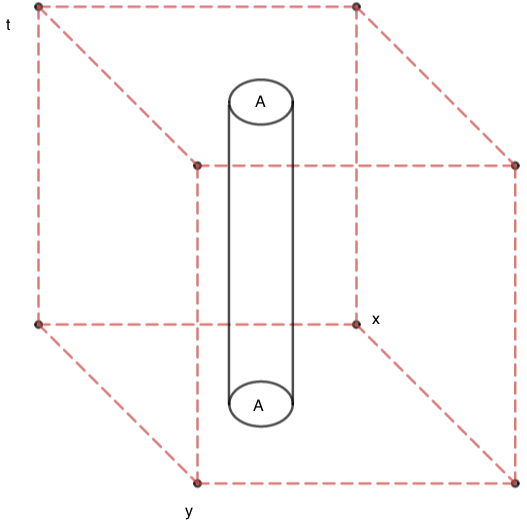
\includegraphics[scale=0.4]{10-3.png}}
            \caption{Drawing for Wangsness 10-3}
        \end{figure}
        \subsubsection{Wangsness 10-6}
        We are given that $\mathbf{P} = P_0 \hat{\mathbf{k}}$. Now $\rho_{b} = -\nabla \cdot \mathbf{P}$, and as $\mathbf{P}$ is uniform, $-\nabla \cdot \mathbf{P} = 0$. Thus $\rho_b = 0$. $\sigma_b = \mathbf{P}\cdot \hat{\mathbf{n}} = P_0 \hat{\mathbf{k}} \cdot \hat{\mathbf{n}} = P_0 \cos(\theta)$. The positive charge is thus located in the region $\theta < \frac{\pi}{2}$. So $Q_b^+ = \int_{0}^{\pi/2}\int_{0}^{2\pi} P_0 \cos(\theta) a^2 \sin(\theta) d\theta d\phi = \pi a^2 P_0$.
        \begin{figure}[htbp]
            \centering
            {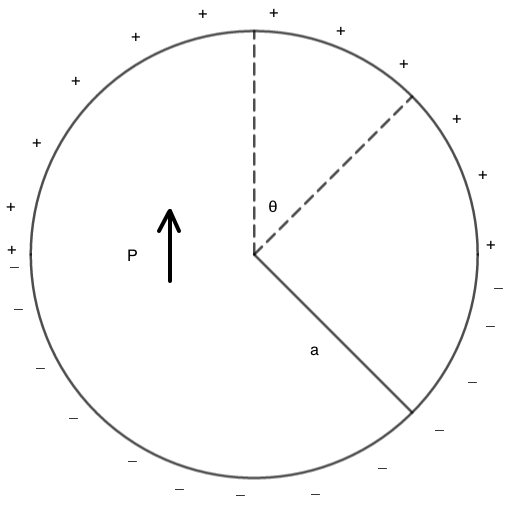
\includegraphics[scale=0.3]{10-6.png}}
            \caption{Drawing for Wangsness 10-6}
        \end{figure}
        \subsubsection{Wangsness 10-17}
        Choose a spherical Gaussian surface outside the sphere concentric with the given sphere. $\int \mathbf{D}\cdot \mathbf{da} = Q_f$, so $D_o (4\pi r^2) = q$, and thus $\mathbf{D}_o = \frac{q}{4\pi r^2} \hat{\mathbf{r}}$. From $\mathbf{D} = \epsilon_0 \mathbf{E}+\mathbf{P}$, we have that $\mathbf{D}_o - \epsilon_0 \mathbf{E}_o = \mathbf{P}_o$. $\mathbf{E}_0 = \frac{q}{4\pi \epsilon_0 r^2}\hat{\mathbf{r}}$, and thus $\mathbf{P}_o = 0$. There is no dielectric outside of the sphere. Choosing a Gaussian surface inside of the sphere, we get $\int \mathbf{D}\cdot \mathbf{da} = Q_f$, for $D(4\pi r^2) = q$, and thus $\mathbf{D}_i = \frac{q}{4\pi r^2} \hat{\mathbf{r}}$. $\mathbf{E}_i = \frac{\mathbf{D}_i}{\epsilon} = \frac{\mathbf{D}_i}{\kappa_e \epsilon_0} = \frac{q}{4\pi \kappa_{e} \epsilon_0 r^2}\hat{\mathbf{r}}$. So $\mathbf{P}_i = \mathbf{D}_i - \epsilon_0 \mathbf{E}_i = (1-\frac{1}{\kappa_{e}}) \frac{q}{4\pi r^2} \hat{\mathbf{r}}$. Finally, $Q_b^{surface} = \int_{S} \sigma_{b} da' = \iint \mathbf{P}\cdot \hat{\mathbf{n}} da' = \int_{0}^{\pi} \int_{0}^{2\pi} \frac{\kappa_e-1}{\kappa_e} \frac{q}{4\pi} \sin(\theta) d\theta d\phi = \frac{\kappa_e-1}{\kappa_e} q$.
        \subsubsection{Wangsness 10-18}
        $\oint \mathbf{D} \cdot \mathbf{da} = q$. $\mathbf{D} = \frac{q}{4\pi r^2} \hat{\mathbf{r}}$ for all $r$ inside the cavity or in the dielectric. $\rho_b = 0$ since $\rho_f = 0$ in the dielectric. In the dielectric $\mathbf{E} = \frac{\mathbf{D}}{\epsilon} = \frac{\mathbf{D}}{\kappa_e \epsilon_0}$, so $\mathbf{E} = \frac{q}{4\pi \kappa_e \epsilon_0 r^2}\hat{\mathbf{r}}$. $\mathbf{P} = \mathbf{D}- \epsilon_0 \mathbf{E} = \frac{\kappa_e-1}{\kappa_e} \frac{q}{4\pi r^2} \hat{\mathbf{r}}$ at the surface of the cavity $r=a$. $\sigma_b = \mathbf{P}\cdot \hat{\mathbf{n}} = \frac{\kappa_e-1}{\kappa_e} \frac{q}{4\pi a^2} \hat{\mathbf{r}}\cdot (-\hat{\mathbf{r}}) = - \frac{\kappa_e-1}{\kappa_e} \frac{q}{4\pi a^2}$. $Q_b^{cavity} = \int \sigma da = - \frac{\kappa_e-1}{\kappa_e}q$.
        \subsubsection{Wangsness 10-25}
        $\kappa_e(x) = \alpha+\beta x$ (The dielectric constant varies linearly with $x$. $\alpha$ and $\beta$ are constants). Find $\mathbf{D}$ between the plates. $\int_{Gaussian Surface} \mathbf{D}\cdot \mathbf{da} = Q_f^{enc}$ (D is uniform between plates). $D\Delta a = Q_f^{enc}$, and thus $D = \frac{Q_f^{enc}}{\Delta a} = \sigma = \frac{Q}{A}$, where $Q$ is the total charge of the plate and $A$ is the area of the plate. $E = \frac{D}{\epsilon} = \frac{Q}{\kappa \epsilon_0 A} = \frac{Q}{\epsilon_0 A(\alpha + \beta x)}$. At $x=0$, $\kappa_e = \kappa_{e_1}$, so $\alpha+\beta(0) = \kappa_{e_1}$, and thus $\alpha = \kappa_{e_1}$. At $x=d$, $\kappa_{e} = \kappa_{e_2}$, and so $\beta = \frac{\kappa_{e_2}-\kappa_{e_1}}{d}$. The potential difference between the plates is $\Delta \phi = -\int_{-}^{+} \mathbf{E}\cdot \mathbf{d\ell} = \int_{+}^{-} Edx = \frac{Q}{\epsilon_0 A} \int_{0}^{d} \frac{dx}{\alpha+\beta x} = \frac{Q}{\epsilon A} \frac{1}{\beta} \ln(\alpha+\beta x)\big|_{0}^{d} = \frac{Q}{\epsilon_0 A\beta} \ln(\frac{\alpha+\beta d}{\alpha}) = \frac{Q}{\epsilon_0 A\beta} \ln(\frac{\kappa_{e_2}}{\kappa_{e_1}}) = \frac{Q}{C}$. Hence $C = \frac{\epsilon_0 A\beta}{\ln(\frac{\kappa_{e_2}}{\kappa_{e_1}})} = \frac{(\kappa_{e_2}-\kappa_{e_1})\epsilon_0 A}{d\ln(\frac{\kappa_{e_2}}{\kappa_{e_1}})}$
        \begin{figure}[H]
          \begin{subfigure}[b]{0.49\textwidth}
             \centering
            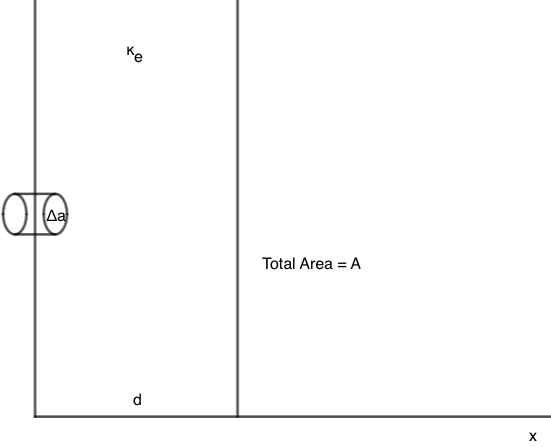
\includegraphics[width=\textwidth]{10-25.png}
            \caption{Drawing for Wangsness 10-25}
          \end{subfigure}
          \begin{subfigure}[b]{0.49\textwidth}
            \centering
            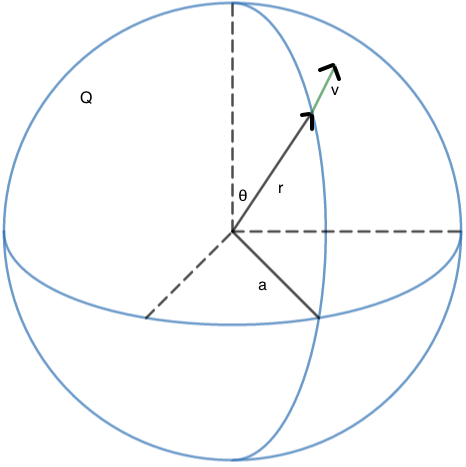
\includegraphics[width=\textwidth]{12-3.png}
            \caption{Drawing for Wangsness 12-3}
          \end{subfigure}
        \end{figure}
        \subsubsection{Wangsness 10-27}
        $\kappa = \kappa_{e_1}$ for $a\leq \rho < \rho_0$, $\kappa = \kappa_{e_2}$ for $\rho_0 \leq \rho \leq b$. First get $D$ by assuming a charge per unit length $\lambda $on the inner cylinder and $-\lambda$ on the outer. $\int \mathbf{D}\cdot \mathbf{da} = Q_{f}^{enc} = D(2\pi \rho L) = \lambda L$. So $\mathbf{D} = \frac{\lambda}{2\pi \rho} \hat{\boldsymbol{\uprho}}$. $\Delta \phi = -\int_{-}^{+} \mathbf{E} \cdot \mathbf{d\ell} = \int_{a}^{b} \frac{\lambda}{2\pi \rho \epsilon}d\rho = \int_{a}^{\rho_0} \frac{\lambda}{2\pi \epsilon_0 \kappa_{e_1}\rho}d\rho + \int_{\rho_0}^{b} \frac{\lambda}{2\pi \epsilon_0 \kappa_{e_2}\rho}d\rho = \frac{\lambda}{2\pi \epsilon_0}\big[\frac{1}{\kappa_{e_1}}\ln(\frac{\rho_0}{a}) + \frac{1}{\kappa_{e_2}}\ln(\frac{b}{\rho_0})\big]$. From $\Delta \phi = \frac{Q}{C}$, and $Q=\lambda L$, we get $C = \frac{2\pi \epsilon_0 L}{\frac{1}{\kappa_{e_1}}\ln(\frac{\rho_0}{a}) + \frac{1}{\kappa_{e_2}}\ln(\frac{b}{\rho_0})}$
\end{document}